\chapter{Introduction}
% See Joel page 3 for 3 main difficulties of EDL
%
%
\section{Motivation}
%Start with Mars landing history (like Guangfei and other dissertation)
NASA has successfully landed five rovers on Mars to date, including the Mars 2020 rover Perseverance. Each of these missions chose low elevation targets between -1 and -4 km relative to the Mars areoid surface, commonly referred to as MOLA, after the instrument that was used to map Mars' topography. 
%Can expand on challenges of entry since I start to talk about it here:
The thin Martian atmosphere makes aerodynamic deceleration ineffective except at lower altitudes where the atmosphere is denser. Coupled with the increasing entry mass required to deliver larger, more capable rovers to the surface, this makes high elevation landing on Mars a challenging problem. Nevertheless, targets above 0 km MOLA, like Terra Sirenum in the Southern Highlands, are motivated by scientific interest~\cite{MarsWater}. In order for descent and landing operations to have sufficient timeline margin~\cite{BraunMarsEDL,MSL_EDL2} when targeting such elevations, the entry phase must be terminated at a sufficiently high altitude.

In addition to altitude, guidance designers must consider other objectives, such as controlling the size of the landing footprint. Both MSL and Mars 2020 had landing ellipse requirements of 25 km x 20 km~\cite{MSL_EDL2,M2020_EDL}. Often these multiple objectives are competing, as for example was the case on the Mars Science Laboratory (MSL) mission, where the entry guidance designers noted that targeting landing site elevations above -1 km MOLA would incur a larger landing ellipse \cite{MSL_EDL2}. 
Future missions, including sample return \cite{MSR} and manned, will place even greater emphasis on robust performance than the current generation, such as pinpoint landing requirements~\cite{PinpointWolf,EvolvableMars}, defined as sub-100 m accuracy. As a component of a possible sample return campaign, Mars 2020 will collect samples for potential return to Earth by a future mission with the campaign, so pinpoint landing is not some far off dream but rather an imminent need. Such a drastic reduction of the footprint will require advances in entry, descent, and landing (EDL) guidance, navigation, and control (GNC). For pinpoint landing, powered descent guidance will be required to ``fly out" dispersions arising during earlier phases, including entry and time spent on the parachute. Powered descent guidance for pinpoint landing has been studied extensively~\cite{PoweredDescentBehcet,PoweredDescentUCI,GFOLDTest,SRP_ControllableSets,PinpointLandingProspects}. 

EDL technology for all previous US Mars landed missions, including MSL and Mars 2020, can trace its heritage to Viking-era space qualification technology from the 1970s~\cite{BraunMarsEDL}. The $ 70^{\circ} $ sphere cone aeroshell used on these missions provides only low lifting capability in the entry phase, during which ballast mass is used to offset the center of mass of the spacecraft to create an angle of attack, thereby generating lift.
The bank angle, which orients the lift vector around the velocity vector, is the control variable by which the vehicle trajectory can be adjusted during the entry phase. Thus, the role of entry guidance is to generate bank angle commands that deliver the vehicle to suitable conditions for descent and landing operations. 
The limited lift available means the control authority is also limited, and as a result, saturation in feedback control is a key issue in Mars entry guidance~\cite{JoelController}.

% Maybe talk briefly about ETPC design here? 

% Maybe segue to talking about how optimal control is the field of extremizing performance. Reference some altitude optimal (and others) papers. Then go to the next section where we discuss the uncertainty, and robust optimal control formulations 
The limited vehicle capability and stringent mission requirements have generated interest in extremizing various performance measures of interest. This is the purview of optimal control theory. Due to the interest in high elevation landings, guidance algorithms designed to maximize altitude at parachute deploy have been studied using optimal control
\cite{HighElevation,AltitudeOptimization,AltitudeOptimizationIndirect,duan2018mars}. 
%Reference \cite{GuangfeiDissertation} proposed an optimization-based onboard trajectory planning method based on a low-order parametrization of the bank angle profile designed to achieve high altitude at parachute deploy.
For hypothetical future missions in which powered descent follows the entry phase directly, i.e., without a parachute phase, propellant-optimal entry guidance has been investigated~\cite{LuAdaptiveEDL,FuelOptimalEndtoEnd,NoyesSRP}

%These first paras set the stage for altitude and range objectives. Next I want to talk about challenges stemming from uncertainty (stochasticity)
In addition to the nominal challenges of Mars EDL, there exists significant uncertainty in the vehicle aerodynamics, initial entry state, and the Martian atmosphere. Thus, in addition to achieving high performance in nominal circumstances, entry guidance must be robust to uncertainty. 
%In the context of pinpoint landing, tighter distributions at the termination of the entry phase allow heavier payloads to be landed by reducing the range of dispersions that powered descent must cover, reducing the total propellant required to be loaded.
One systematic way to balance nominal performance and robustness is to formulate an optimal control that weights a nominal (or mean) optimization objective with minimization of a function of the state covariance matrix.
Throughout this dissertation, we refer to such optimal control formulations as robust optimal control problems (ROCP)~\cite{RobustOptimalControl}. There appears to be no standard nomenclature in the literature, where such problems are also sometimes referred to as uncertain optimal control~\cite{PhelpsUncertainOCP}, optimal trajectory design under uncertainty~\cite{EntryOUUThesis2,darlington2000decreasing}, Riemann-Stieljtes optimal control~\cite{RossRSOCP}, and more. Due to the close relationship between the sensitivity matrix (also called the state transition matrix) and the state covariance matrix, we also include desensitized optimal control \cite{Desensitized,TrajectoryDesensitization} under the umbrella of robust optimal control. Figure~\ref{Fig:RobustTrajectoryOpt} depicts the concept of Mars entry as an ROCP. 
\begin{figure}[h!]
	\centering
	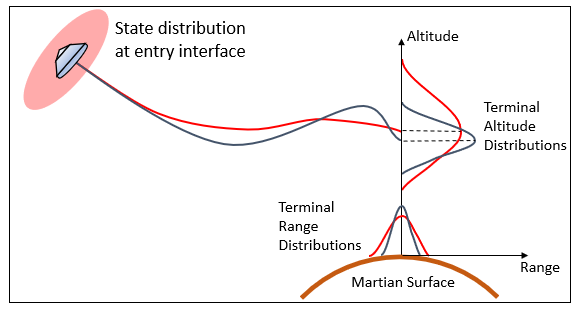
\includegraphics[width=0.8\textwidth]{Images/RobustTrajectoryOptimization}
	\caption{The concept of robust optimal control.}
	\label{Fig:RobustTrajectoryOpt}
\end{figure}

Approaches to entry guidance based on robust optimal control have been studied in \cite{AltitudeUnderUncertainty, EntryOUUThesis1, EntryOUUThesis2, MarsEntryDesensitized, EntryOUU}. 
The literature on ROCPs can be divided into open- and closed-loop control strategies. Open-loop solutions to ROCPs have been proposed when feedback is unavailable~\cite{RossRSOCP}, or for use as a reference trajectory in closed-loop trajectory tracking~\cite{EntryOUUThesis1}. Open-loop covariance shaping relies on nonlinearities of the system models; for linear systems, the state covariance does not depend on the mean state, and thus in the absence of feedback, no covariance shaping can be performed. References~\cite{AltitudeUnderUncertainty,EntryOUUThesis1} explored open-loop robust optimal control for entry guidance, where only the path through the atmosphere is used to effect change on the terminal state covariance. In closed-loop ROCPs, a feedback control law $\control(t,\state)$ is modeled. Closed-loop solutions to ROCPs have been discussed in the context of entry in \cite{EntryOUUThesis2} and \cite{MarsEntryDesensitized}. 

%No guarantee of good performance doing this; we can cite a counterexample where w_h=w_s=0, the open loop optimal is basically bang-bang, terrible margins.
A key reason to differentiate between open- and closed-loop is due to constraints on the control variables. 
In open-loop ROCP, path constraints on the controls are treated in the deterministic fashion. That is, because the control is purely a function of the independent variable, enforcing a general nonlinear constraint for the nominal trajectory ensures it is satisfied for any trajectory. 
In closed-loop formulations, one way to proceed is to treat the constraint as a probabilistic chance constraint, which ensures the constraint is satisfied with at least some chosen probability. However, control constraints are often related to hard physical limits, such as the maximum thrust available to a spacecraft, and probabilistic satisfaction may not be appropriate. The most common examples are norm-bounded controls, and individual control limits. To strictly enforce such constraints, a new piecewise continuous control can defined by treating the constraint as part of the feedback control law such that the control constraint is guaranteed to be satisfied. As a result of the hard enforcement in the ROCP, the optimal controls will balance the distance of the open-loop controls from the constraint in order to balance the mean performance and robustness as measured by some function of the state variance.

All of the existing applications of robust optimal control to entry guidance have utilized linear methods of determining the state covariance or sensitivity matrices, and little discussion of the effects of control saturation are found among the references. Control saturation is a nonlinear, non-differentiable phenomenon. A natural question is whether linear methods are sufficiently accurate in the presence of control saturation. Due to the limited control authority of Mars entry vehicles, we incorporate hard control saturation in our problem model, and as a consequence also consider whether or not linear methods are appropriate for our goals.
%This does make the control non-differentiable at the control bounds. 



%A key reason to differentiate between open- and closed-loop is due to constraints on the control variables. 
%In open-loop ROCP, path constraints on the controls are treated in the deterministic fashion. That is, because the control is purely a function of the independent variable, $\control(t,\state)=\control(t)$, enforcing a general nonlinear constraint $c(\control(t))\le0$ for the nominal trajectory ensures it is satisfied for any trajectory. 
%In closed-loop formulations, the same path constraint $c(\control(t,\state))\le0$ may be impossible to enforce $\forall\,\state\in\mathbb{X}$. One way to proceed is to treat the constraint as a probabilistic chance constraint, $\mathbb{P}[c(\control(t,\state))\le0] \ge p$, which ensures the constraint $c$ is satisfied with at least probability $p$. However, control constraints are often related to hard physical limits, such as the maximum thrust available to a spacecraft, and probabilistic satisfaction may not be appropriate. The most common examples are norm-bounded controls $||\control|| < u_{\max}$, and individual control limits $u_{\min}\le u_i \le u_{\max}$. To strictly enforce such constraints, a new piecewise continuous control can defined by treating the constraint as part of the feedback control law. For example, in the latter case of a bounded scalar control, we can define 
%\begin{align*}
%\tilde{u}(t,x) = \begin{cases}
%u_{\min} & u(t,x) < u_{\min}\\
%u(t,x) & u_{\min}\le u \le u_{\max} \\
%u_{\max} & u(t,x) < u_{\max}
%\end{cases}
%\end{align*}
%and as a result, regardless of the how the control $u(t,x)$ is parametrized, the control constraint is guaranteed to be satisfied.
%
%All of the existing applications of robust optimal control to entry guidance have utilized linear methods of determining the state covariance or sensitivity matrices, and little discussion of the effects of control saturation are found among the references. Control saturation is a nonlinear, non-differentiable phenomenon. A natural question is whether linear methods are sufficiently accurate in the presence of control saturation. Due to the limited control authority of Mars entry vehicles, we incorporate control saturation in our problem model, and as a consequence also consider whether or not linear methods are appropriate for our purposes.
%%This does make the control non-differentiable at the control bounds. 

% There are a number of key difference between the probabilist control constraint and the hard constraint. The first is that the user must choose, a priori, the probability of control saturation. It is unclear how such a value should be set to produce optimal results. The hard constraint formulation instead allows the solution to saturate to the degree that is optimal for the performance index. In this sense, the probabilistic constraint is actually more restrictive. Additionally with the hard constraint, the degree of saturation can (and naturally, does) vary throughout the trajectory. 

%Depending on how the control law is parametrized, there may be no way to enforce such a constraint within the optimization process. However, the constraint can instead be absorbed into the definition of the control law, and treated as an additional nonlinearity in the dynamics. To make this idea more concrete, consider an affine state-feedack, $u(t,\state) = u_0(t) + K(t)\state(t)$, and a normally distributed state, $\state\sim\normal(\bar{\state},\cov_{\state})$. We have $\E{u} = u_0 + K(t)\bar{\state}$ and $\V{u} = \E{u^2}-\E{u}^2=K\cov_{\state}K^T$. $\mathbb{P}[u_{\min}\le u \le u_{\max}] = F(u_{\max})-F(u_{\min})$. Even if the optimizer is free to choose the functions $u(t)$ and $K(t)$.

%Reference~\cite{EntryOUUThesis1} explored the relationship between covariance reduction and sensitivity reduction, and ultimately recommended the covariance formulation for several reasons, including smaller problem size due to the symmetry of the covariance matrix, the ability to incorporate measurements, and simpler formulation and interpretation of variances compared to elements of the sensitivity matrix.

For current generation missions using parachute-based EDL, we restrict our attention to the same class of guidance law as Mars 2020, affine state-feedback.
The specific objectives of this dissertation are 1) for given models of the vehicle and planet (including parametric uncertainty), determine a reference control, reference trajectory, and feedback gains that, when used for closed-loop reference tracking guidance, will optimize a performance index chosen based on mission requirements, and 2) to enable fast, efficient guidance design that is free of computationally expensive Monte Carlo simulations in the loop and hand tuning of key guidance parameters. This is motivated by the approach used for MSL, in which design maps are generated via iteration over guidance parameters with Monte Carlo simulation performed for each combination of parameters. A more detailed review of the MSL design process in deferred to Section~\ref{Sec:ETPC}.
% Finally, we consider how the role of entry guidance might change in parachute-free, SRP-based EDL. The 3rd objective is to develop an algorithm

To meet our first objective, this dissertation builds on the robust optimal control approach to entry guidance.
Our formulation differs from the existing formulations in the form of our performance index, the use of velocity as the independent variable, and, in light of the previous discussion, careful consideration of the limited control authority and the effects of control saturation on the state distribution.

The solution of nonlinear optimal control problems is, in general, not a simple task. Add to that the complexity of quantifying uncertainty at each iteration of the solution process, and it is easy to see that solving ROCPs is a challenging problem. To meet our second objective, we propose and demonstrate an efficient solution method for the entry guidance ROCP based on Differential Dynamic Programming (DDP) and the Unscented Transform (UT). The UT is chosen because it is better suited to propagating the mean and state covariance through the nonlinear dynamics than linear methods. A numerical example is given to illustrate this point. DDP is chosen for its suitability to large-scale optimal control problems, and its robust convergence properties. Starting from the control-limited DDP algorithm presented in~\cite{DDP_ControlLimited}, we examine an iterated Linear-Quadratic-like simplification~\cite{iLQG} that is enabling in solving the ROCP. Next, we extend the algorithm to jointly optimize the static feedback gains concurrently with the reference control for improved performance. Using the MSL and Mars 2020 missions as our benchmark, the performance of the guidance solutions is assessed numerically. 



%\subsection{Other Approaches to Entry Guidance}
%
%The ETPC represents the current practice in Mars entry guidance but many alternative entry guidance algorithms have been proposed. There are many ways that algorithms can be characterized and categorized. One popular delineation is between methods that utilize a pre-planned reference trajectory, and those that do not. In the first category are explicit reference tracking approaches, in which a feedback law attempts to keep the vehicle state close to the reference state. Many nonlinear control techniques, such as feedback linearization~\cite{FeedbackLinearization}, nonlinear predictive control~\cite{NMPC,JoelController} and sliding mode control~\cite{SlidingModeEG1} have been applied to reference tracking guidance. 
%One advantage of reference-based solutions is the flexibility in designing the reference trajectory before flight, allowing for intensive computations not suitable for in-flight operations. Guidance solutions generated by solving ROCPs, like those discussed earlier, fall into this category. Reference trajectory-based approaches also have some degree of model independence~\cite{joel_dissertation}.
%
%In the category of reference-free guidance are computational approaches, including predictor-corrector guidance~\cite{EntryPredictCorrect}, and convex optimization~\cite{MaxCrossrangeConvexLu,ConvexEntryGuidance}. These methods have higher computational complexity and model dependence, but may also offer higher performance. In Chapters~\ref{Ch:FuelOptimalPaper} and \ref{Ch:FuelOptimalAssessment} we propose a predictor-corrector guidance for future Mars missions.
%
%Many entry guidance algorithms defy categorization along these lines, or blur the line between these approaches. For instance, the ETPC does make use of a reference trajectory, but not does track it directly. Instead, the reference trajectory is used to determine sensitivities, called influence coefficients, that allow the guidance to steer the vehicle along a neighboring path that ends at the same range at a fixed velocity. Because the ETPC makes a prediction of the terminal range and corrects based on the predicted error, it is sometimes called an analytical predictor-corrector. There are also a number of proposed methods for onboard updating of reference trajectories~\cite{GuangfeiReplanning} that naturally have elements of both reference tracking and computational guidances.  

% Refences with notes:
% AltitudeUnderUncertainty
% MarsEntryDesensitized % linearized but closed-loop with fixed gain. No consideration of saturation 
% EntryOUU % Does not use linearization, also doesnt solve in a conventional way, maybe remove?
% TrajectoryDesensitization % Desensitized like seywald and kumar, is it entry applied?
% EntryOUUThesis1 % Earth EDL, focuses on footprint computation, only considers open-loop in the reentry problem, and did not conduct monte carlo to confirm
% EntryOUUThesis2 % LQR, minimum control effort objective which stays away from the bounds, angle of attack as control variable. Does perform Monte Carlo(s) to validate improvement. 

% Introduction to my approach? 
% State the specific objective(s) of my research 
% One goal is efficient solution 
% One goal is good guidance performance in simulations


%The specific objective of this dissertation are to design an entry guidance with the same computational complexity as the state-of-the-practice guidance algorithm while providing superior performance. 

\section{Dissertation Organization}
This remainder of this dissertation is organized as follows: The remainder of this chapter further reviews the state-of-the-practice guidance flown on MSL and Mars 2020. 

Chapter~\ref{Ch:EGConcepts} begins with an overview of the EDL timeline. A high level discussion of the entry guidance problem, especially target conditions, is presented.

Chapter~\ref{Ch:Models} discusses the models of the vehicle and environment used to derive the guidance algorithm.

Chapter~\ref{Ch:GuidanceStrategy} outlines the guidance strategy, including formally posing the problem as a ROCP.

Chapter~\ref{Ch:SolutionMethod} discusses uncertainty quantification and presents a numerical example demonstrating the benefit of UT depending on whether the control strategy is open-loop or closed-loop. An algorithm based on constrained DDP is modified to solve the ROCP. Two modifications to the ROCP are made in order for the DDP algorithm to be applicable. 

Chapter~\ref{Ch:AssessmentConditions} presents the assessment conditions, including algorithm parameters, details of the Monte Carlo simulations. 

Chapter~\ref{Ch:NumericalAssessment} presents an assessment of the guidance algorithm for MSL-class vehicle.  A negative result associated with joint optimization of velocity-varying feedback control gains is presented. Chapter~\ref{Ch:SRL_EDL} presents a similar assessment for a heavier vehicle in the class of the Sample Retrieval Lander.

In Chapter~\ref{Ch:FuelOptimalPaper} we direct our attention to chuteless, SRP-based EDL envisioned for future missions. A numerical predictor-corrector entry guidance algorithm is developed to minimize the predicted propellant during the powered descent phase. Chapter~\ref{Ch:FuelOptimalAssessment} presents a numerical assessment of the guidance approach. 

In Chapter~\ref{Ch:Conclusions} the conclusions are stated, and several avenues for future work are discussed.

%\section{Entry Guidance Review}
\section{Entry Terminal Point Controller}\label{Sec:ETPC}
The state-of-the-practice for Mars entry guidance, used on MSL and Mars 2020, is a modified version of the Apollo command module entry guidance \cite{MSL_EDL2} called the entry terminal point controller (ETPC). 
The three phases of the ETPC are prebank, range control, and heading alignment. In the prebank phase, there is no guidance, but the vehicle is rotated to the expected initial bank angle for the start of the range control phase.
The range control guidance begins when the sensed drag deceleration exceeds a threshold value, and consists of longitudinal guidance and lateral guidance. Longitudinal guidance modulates the bank angle magnitude to control the range flown, and reduce range dispersions at parachute deployment. Lateral guidance operates concurrently with longitudinal guidance during range control to command bank reversals when a measure of the crossrange to the target exceeds the deadband threshold, which is a quadratic function of velocity. At a specified velocity, the guidance switches from range control to heading alignment, during which the bank angle is commanded to reduce the crossrange error. During heading alignment, the bank angle magnitude is restricted to $30^{\circ}$. This ensures that most of the lift vector is opposite gravity, which results in increased parachute deploy altitude.
For MSL and Mars 2020, the vehicle was required to land in an ellipse of $25$ km $\times 20$ km~\cite{MSL_EDL2,M2020_EDL}. Due to the expansion of the ellipse during time spent on the parachute, the entry guidance requirement was to deploy the parachute with 10 km of the planned parachute deploy target~\cite{MSL_EDL2}. The ETPC delivered MSL to an elevation of -4.4 km with a target miss distance of 2.3 km and a 99\% confidence landing ellipse of 19.1 km $\times$ 6.9 km~\cite{MSL_EDL2}.

%As its name implies, the purpose of the longitudinal range control is to reduce range errors. Lateral guidance indirectly manages crossrange error during range control, while heading alignment reduces crossrange errors until the sequence leading to parachute deploy is initiated. Thus in the design for MSL, achieving sufficient terminal altitude is accomplished primarily by the choice of the reference trajectory, and numerical simulations were performed to show the range control guidance did not result in lower parachute deploy altitude. 

The entry guidance for these latest Mars entry vehicles \cite{MSL_EDL2,M2020_EDL} is designed by multiple iterations of two steps. The first step is to design a reference bank profile and compute the corresponding reference trajectory via open-loop simulation. The reference bank angle profile is specified by a small number of parameters, a modification from the original Apollo algorithm, which assumed a constant bank angle reference profile. This change allows for more flexibility in trajectory design, including enabling higher parachute deploy altitudes \cite{MSL_EDL2}. Because the ETPC range control feedback gains depend on the reference trajectory~\cite{Apollo}, the flexibility in the design of the reference trajectory is the primary means of affecting the overall performance of range control. The parameters specifying the reference control must be chosen to provide control margin for both longitudinal and lateral guidance, while also achieving high altitude.
In the second step, some of the more severe off-nominal entries are simulated in closed-loop using the reference trajectory, ETPC gains, and heading alignment guidance to estimate off-nominal performance prior to Monte Carlo simulation \cite{MSL_EDL2}. The results are judged based on the vehicle state at parachute deployment. The free parameters of the guidance algorithm, including the overcontrol gain and heading alignment gain, are then tuned as necessary to improve the performance. When the required performance cannot be achieved through tuning, the reference trajectory is changed and the process repeats. The iterative two-step process ends up requiring consideration of 100s or 1000s of reference trajectories \cite{MSL_EDL2}. Eliminating this iterative process is a key objective of this dissertation.
%The longitudinal range control guidance uses linear gains computed by the adjoint equations to find a neighboring optimal path that terminates at the same range as the reference trajectory. 

In Chapter~\ref{Ch:GuidanceStrategy}, we propose an alternative to the longitudinal guidance operating during the range control phase. However, because our alternative guidance does not focus exclusively on range, we prefer to refer to it as second phase guidance. Similarly, the third phase guidance for MSL and Mars 2020 was heading alignment guidance, and alternative third phase guidance approaches has been proposed~\cite{GuangfeiDissertation}.



% Reference updating approaches? Also blur the line sicne they use reference but also are computational for onbaord updating...


%%% Local Variables: ***
%%% mode: latex ***
%%% TeX-master: "thesis.tex" ***
%%% End: ***
